\documentclass{standalone}
\usepackage{tikz}
\usepackage{calc}
\usepackage{pgffor}
\usetikzlibrary{patterns}
\begin{document}
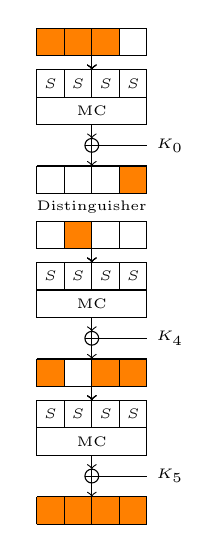
\begin{tikzpicture}[scale=0.35]
\begin{scope}[yshift = -5cm]
\fill[orange](3,0) rectangle+(1,1);
\end{scope}
\begin{scope}[yshift = 0cm]
\fill[orange](0,0) rectangle+(1,1);
\fill[orange](1,0) rectangle+(1,1);
\fill[orange](2,0) rectangle+(1,1);
\end{scope}
\begin{scope}[yshift = -7cm]
\fill[orange](1,0) rectangle+(1,1);
\end{scope}
\begin{scope}[yshift = -12cm]
\fill[orange](0,0) rectangle+(1,1);
\fill[orange](2,0) rectangle+(1,1);
\fill[orange](3,0) rectangle+(1,1);
\end{scope}
\begin{scope}[yshift = -17cm]
\fill[orange](0,0) rectangle+(1,1);
\fill[orange](1,0) rectangle+(1,1);
\fill[orange](2,0) rectangle+(1,1);
\fill[orange](3,0) rectangle+(1,1);
\end{scope}
\begin{scope}[yshift =0 cm]
\draw (0,0) grid +(4,1);
\foreach \y in {0,1,2,3}{\draw[->](2,0)--+(0,-0.5);
\draw(\y,-1.5) rectangle node{\tiny{$S$}} +(1,1);
}
\draw (0,-2.5) rectangle node{\tiny{MC}} +(4,1);
\draw[->] (2,-2.5)--+(0,-0.5);
\draw (1.75,-3.25)--+(0.5,0);
\draw (2,-3.25) circle (0.25);
\draw (4,-3.25) --(2.25,-3.25);
\node[right] at (4,-3.25) {\tiny{$K_0$}};
\draw[->](2,-3)--+(0,-1);
\end{scope}
\draw(0,-5) grid +(4,1);
\node at (2,-5.5){\tiny{Distinguisher}};
\begin{scope}[yshift =-7 cm]
\draw (0,0) grid +(4,1);
\foreach \y in {0,1,2,3}{\draw[->](2,0)--+(0,-0.5);
\draw(\y,-1.5) rectangle node{\tiny{$S$}} +(1,1);
}
\draw (0,-2.5) rectangle node{\tiny{MC}} +(4,1);
\draw[->] (2,-2.5)--+(0,-0.5);
\draw (1.75,-3.25)--+(0.5,0);
\draw (2,-3.25) circle (0.25);
\draw (4,-3.25) --(2.25,-3.25);
\node[right] at (4,-3.25) {\tiny{$K_4$}};
\draw[->](2,-3)--+(0,-1);
\end{scope}
\begin{scope}[yshift =-12 cm]
\draw (0,0) grid +(4,1);
\foreach \y in {0,1,2,3}{\draw[->](2,0)--+(0,-0.5);
\draw(\y,-1.5) rectangle node{\tiny{$S$}} +(1,1);
}
\draw (0,-2.5) rectangle node{\tiny{MC}} +(4,1);
\draw[->] (2,-2.5)--+(0,-0.5);
\draw (1.75,-3.25)--+(0.5,0);
\draw (2,-3.25) circle (0.25);
\draw (4,-3.25) --(2.25,-3.25);
\node[right] at (4,-3.25) {\tiny{$K_5$}};
\draw[->](2,-3)--+(0,-1);
\end{scope}
\draw (0,-17) grid +(4,1);
\end{tikzpicture}
\end{document}